
\chapter{Polinomios de Taylor}



\section{Introducción y Definición}

Sea $p(x)$ un polinomio de grado $n$, es decir
\[
 p(x) = a_0 + a_1 x + a_2 x^2 + \dots + a_{n-1} x^{n-1} + a_n x^n.
\]
Nos preguntamos: ¿Qué relación existe entre las derivadas de $p$ en $x = 0$ y el valor de los coeficientes $a_i$?
Veamos:
\begin{align*}
 p(0)   &= a_0 \\
 p'(x)  &= a_1 + 2 \cdot a_2 \cdot x + 3 \cdot a_3 \cdot x^2 + \dots + (n-1) \cdot a_{n-1} \cdot x^{n-2} + n \cdot a_n \cdot x^{n-1} \\
 p'(0)  &= a_1 \\
 p''(x) &= 2 \cdot a_2 + 3 \cdot 2 \cdot a_3 \cdot x + \dots + (n-1) \cdot (n-2) \cdot a_{n-1} \cdot x^{n-3} + n \cdot (n-1) \cdot a_n \cdot x^{n-2} \\
 p''(0) &= 2 \cdot a_2 \\
 p'''(x) &= 3\cdot 2 \cdot a_3 + \dots + (n-1) \cdot (n-2) \cdot (n-3) \cdot a_{n-1} \cdot x^{n-4} + n \cdot (n-1) \cdot (n-2) \cdot a_n \cdot x^{n-3} \\
 p'''(0) &= 3 \cdot 2 \cdot a_3 \\
&\ \,\vdots
\end{align*}
Vemos entonces (y se puede demostrar por inducción) que
\[
 p^{(k)} (0) = k! \, a_k,\qquad k=0,1,2,\dots.
\]
Notar que si el polinomio es de grado $n$, entonces $p^{(n+1)}(x) = 0$ para todo $x \in \R$.

Concluimos que

\recuadro{%
Si $p(x)$ es un polinomio de grado $n$, entonces
\[
 p(x) = p(0) + p'(0) \, x + \frac{p''(0)}{2!}\, x^2 + \frac{p'''(0)}{3!}\, x^3 + \dots
 %+ \frac{p^{(n-1)}(0)}{(n-1)!} \, x^{n-1} 
+ \frac{p^{(n)}(0)}{n!} \, x^{n}.
\]
}

Hemos descrito un polinomio en base al valor de sus derivadas en $x=0$.
Análogamente, podemos describir un polinomio en términos del valor de sus derivadas en $x=a$, para cualquier número real fijo $a$:

\recuadro{%
Si $p(x)$ es un polinomio de grado $n$, entonces
\[
 p(x) = p(a) + p'(a) \, (x-a) + \frac{p''(a)}{2!}\, (x-a)^2 + \frac{p'''(a)}{3!}\, (x-a)^3 + \dots
% + \frac{p^{(n-1)}(a)}{(n-1)!} \, (x-a)^{n-1} 
+ \frac{p^{(n)}(a)}{n!} \, (x-a)^{n}.
\]
}

Motivados por esta igualdad, definimos

\begin{definition}[Polinomio de Taylor]
 Si $f$ es una función $n$ veces derivable en $x=a$, se llama \emph{polinomio de Taylor} de $f$, de orden $n$ alrededor de $x=a$ al polinomio:
\[
 p_n(x) = f(a) + f'(a) \, (x-a) + \frac{f''(a)}{2!}\, (x-a)^2 + \frac{f'''(a)}{3!}\, (x-a)^3 + \dots
% + \frac{f^{(n-1)}(a)}{(n-1)!} \, (x-a)^{n-1}
 + \frac{f^{(n)}(a)}{n!} \, (x-a)^{n}.
\]
Es decir, el polinomio de Taylor de $f$ de orden $n$ alrededor de $x=a$ es el único polinomio de grado $n$ tal que el valor del mismo y de sus primeras $n$ derivadas en $x=a$ coincide, respectivamente, con el valor de $f$ y de sus primeras $n$ derivadas en $x=a$.
\end{definition}

\begin{example}
 Hallar el polinomio de Taylor de orden 4 de $f(x) = e^x$ alrededor de $x=0$.

 Para ello, debemos calcular $f(0)$, $f'(0)$, $f''(0)$, $f'''(0)$, $f^{(4)}(0)$:
\[
\begin{aligned}
 f(x) &= e^x  \quad &\Longrightarrow & &\quad f(0)  &= 1 \\
 f'(x) &= e^x \quad &\Longrightarrow& & \quad f'(0) &= 1 \\
 f''(x) &= e^x \quad &\Longrightarrow& & \quad f''(0) &= 1 \\
 f'''(x) &= e^x \quad &\Longrightarrow& & \quad f'''(0) &= 1 \\
 f^{(4)}(x) &= e^x \quad &\Longrightarrow& & \quad f^{(4)}(0) &= 1 \\
\end{aligned}
\]
Por lo tanto 
\[
 p_4(x) = 1 + 1 \cdot x + \frac{1}{2!} \cdot x^2 + \frac{1}{3!} \cdot x^3 +  \frac{1}{4!} \cdot x^4 .
\]
Puede verse que para esta función particular, $f^{(k)}(0) = 1$ para todo $k \in \N$, y por lo tanto, cualquiera sea $n\in\N$, el polinomio de Taylor de orden $n$ de $f(x) = e^x$ alrededor de $x=0$ es
\begin{align*}
 p_n(x) &= 1 + 1 \cdot x + \frac{1}{2!} \cdot x^2 + \frac{1}{3!} \cdot x^3 +\dots +  \frac{1}{n!} \cdot x^n \\
&= 1 +  x + \frac{x^2}{2!} + \frac{1}{3!} \cdot x^3 + \dots +  \frac{x^n}{n!}  \\
&= \sum_{k=0}^n \frac{x^k}{k!}.
\end{align*}
\end{example}

\begin{center}
  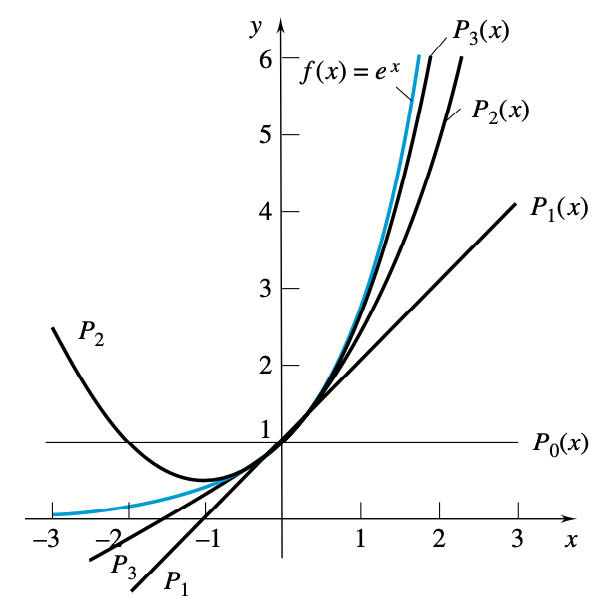
\includegraphics[width=.4\textwidth]{pics/taylor-exp.png}
  \hfil
  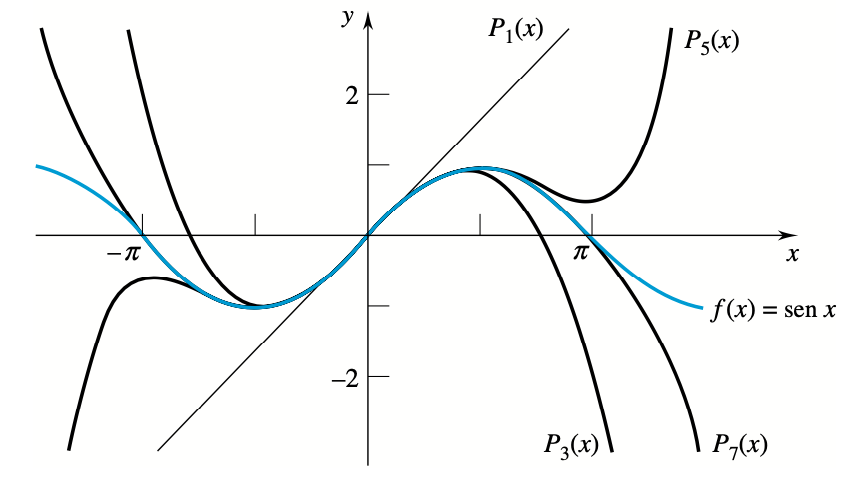
\includegraphics[width=.59\textwidth]{pics/taylor-sen.png}
\end{center}

\begin{example}
Hallar el polinomio de Taylor de $f(x) = \sen(x)$ de orden 6 alrededor $x=0$.
Observemos que
\[
\begin{aligned}
 f(x) &= \sen(x)  \quad &\Longrightarrow & &\quad f(0)  &= 0 \\
 f'(x) &= \cos(x) \quad &\Longrightarrow& & \quad f'(0) &= 1 \\
 f''(x) &= -\sen(x) \quad &\Longrightarrow& & \quad f''(0) &= 0 \\
 f'''(x) &= -\cos(x) \quad &\Longrightarrow& & \quad f'''(0) &= -1 \\
 f^{(4)}(x) &= \sen(x) \quad &\Longrightarrow& & \quad f^{(4)}(0) &= 0 \\
 f^{(5)}(x) &= \cos(x) \quad &\Longrightarrow& & \quad f^{(5)}(0) &= 1 \\
 f^{(6)}(x) &= -\sen(x) \quad &\Longrightarrow& & \quad f^{(6)}(0) &= 0 
\end{aligned}
\]
Por lo tanto
\begin{align*}
p_6(x) &= 0 + 1 \cdot x + \frac{0}{2!} \cdot x^2 + \frac{-1}{3!} \cdot x^3 +
          \frac{0}{4!} \cdot x^4 + \frac{1}{5!} \cdot x^5 + \frac{0}{6!} \cdot x^6 \\
       &= x - \frac{x^3}{3!} + \frac{x^5}{5!}.
\end{align*}
Y vemos que en general
\[
p_n(x) =  x - \frac{x^3}{3!} + \frac{x^5}{5!} - \frac{x^7}{7!} + \frac{x^9}{9!} - \frac{x^11}{11!} + \dots
          + (-1)^{k+1} \frac{x^{2k-1}}{(2k-1)!},
\]
con $k$ el mayor entero tal que $2k-1 \le n$, es decir $k = \left\lfloor \frac{n+1}2 \right\rfloor$.
\end{example}

\begin{example}
 Hallar el polinomio de Taylor de $f(x) = \ln (x)$ de orden $5$ alrededor de $x=1$. 
Observemos que
\[
\begin{aligned}
 f(x) &= \ln(x)  \quad &\Longrightarrow & &\quad f(1)  &= 0 \\
 f'(x) &= \frac{1}{x} \quad &\Longrightarrow& & \quad f'(1) &= 1 \\
 f''(x) &= -\frac{1}{x^2}\quad &\Longrightarrow& & \quad f''(1) &= -1 \\
 f'''(x) &= \frac{2}{x^3} \quad &\Longrightarrow& & \quad f'''(1) &= 2 \\
 f^{(4)}(x) &= -\frac{2\cdot 3}{x^4} \quad &\Longrightarrow& & \quad f^{(4)}(1) &= -2 \cdot 3 \\
 f^{(5)}(x) &= \frac{2\cdot 3 \cdot 4}{x^5} \quad &\Longrightarrow& & \quad f^{(5)}(1) &= 2 \cdot 3\cdot 4 
\end{aligned}
\]
Por lo tanto
\begin{align*}
p_5(x) &= 0 + 1 \cdot (x-1) + \frac{-1}{2!} \cdot (x-1)^2 + \frac{2}{3!} \cdot (x-1)^3 +
          \frac{-2 \cdot 3}{4!} \cdot (x-1)^4 + \frac{2\cdot 3\cdot 4}{5!} \cdot (x-1)^5\\
       &= (x-1) - \frac{(x-1)^2}{2} + \frac{(x-1)^3}{3} - \frac{(x-1)^4}{4} + \frac{(x-1)^5}{5}.
\end{align*}
¿Puede imaginarse la forma del polinomio de Taylor de orden $n$ en este caso?
\end{example}

\subsection*{Interpretación geométrica}

Para ver qué representa geométricamente el polinomio de Taylor de una cierta función de grado $n$ alrededor de un punto dado, consideramos como ejemplo la función $f(x) = \sen(x)$ y graficamos en un mismo par de ejes, la función dada y sus polinomios de Taylor de orden 0 a 4 alrededor de $x=0$

\centerline{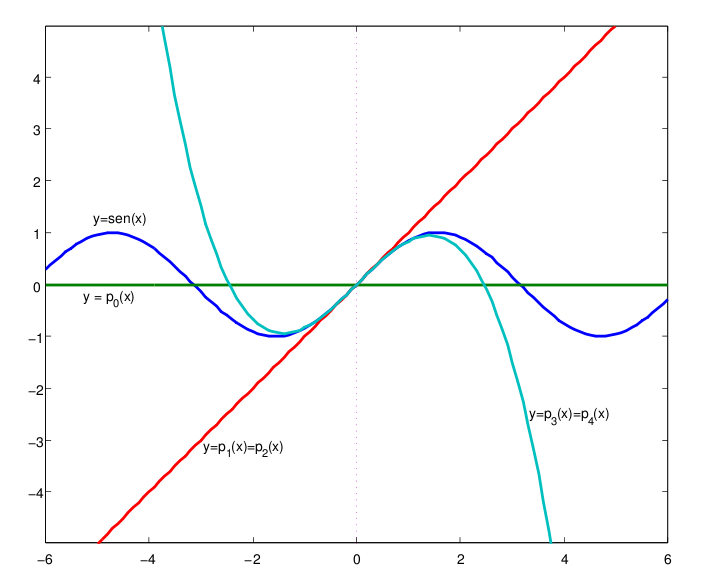
\includegraphics[width=.6\textwidth]{pics/taylor-seno-1.png}}

Lo primero que observamos es que $p_0(x)$ es una recta horizontal que coincide con la función en $(0, f(0))$. El polinomio $p_1(x)$ es lineal y tanto su valor como el valor de su derivada coinciden con los de $f$ en $x=0$, por lo tanto la gráfica de $p_1(x)$ es la recta tangente a la gráfica de $f(x)$ en $(0,f(0))$. Para este ejemplo, el polinomio $p_2(x)$ coincide con $p_1(x)$ porque $f''(0) = 0$.

También observamos que a medida que aumentamos el orden del polinomio de Taylor, estos aproximan cada vez mejor a la función. A continuación graficamos la misma función y sus polinomios de Taylor de orden 5 a 10. 

\centerline{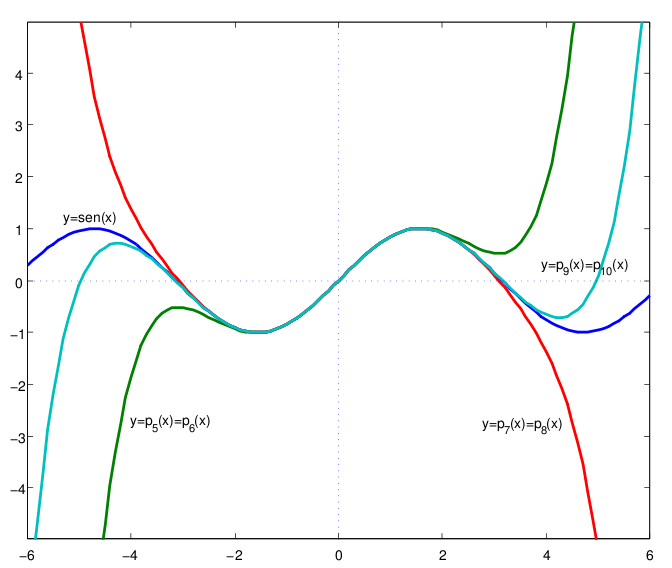
\includegraphics[width=.6\textwidth]{pics/taylor-seno-2.png}}

Vemos que a medida que aumenta el orden la aproximación mejora pues las graficas se mantienen cerca de la gráfica de $y=\sen(x)$ en intervalos más grandes.

También observamos que lejos de $x=0$ la aproximación es mala, pues todo polinomio $p(x)$ no-constante satisface $\lim_{x\to\infty} p(x) = \infty$.

\subsection*{Un ejemplo interesante}
Por otro lado, si consideramos la función 
\[
 f(x) = \begin{cases}
         e^{-1/x^2} \quad &\text{si } x \neq 0 \\
         0          \quad &\text{si } x = 0 
        \end{cases}
\]
resulta que tiene todas sus derivadas nulas en $x = 0$, es decir
\[
 f'(0) = 0, \quad f''(0) = 0, \quad f'''(0) = 0,\quad  \cdots, \quad f^{(n)}(0) = 0, \quad \cdots
\]
Por lo tanto, el polinomio de Taylor alrededor de $x = 0$ es el polinomio nulo $p_n(x) \equiv 0$ para cualquier $n$.
En este caso no es cierto que $p_n(x)$ se aproxime cada vez más a $f(x)$ a medida que $n$ crece.

\centerline{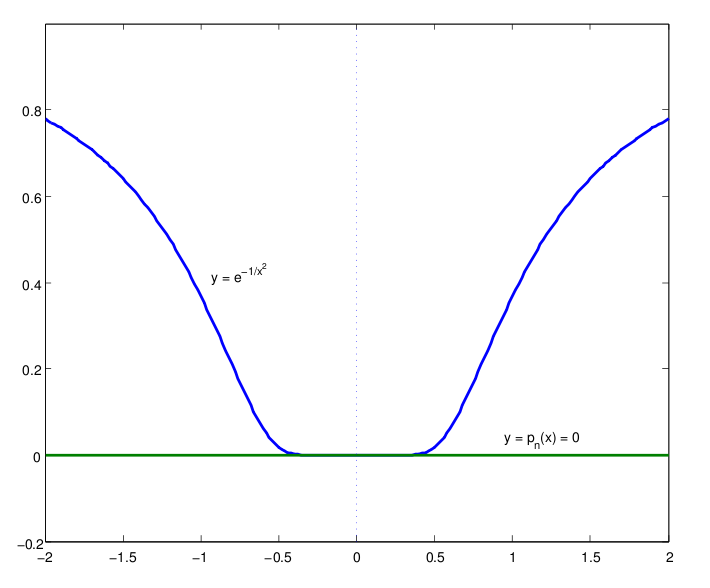
\includegraphics[width=.6\textwidth]{pics/taylor-patologico.png}}



\subsubsection*{Ejercicios de la sección~\getcurrentref{chapter}.\getcurrentref{section}}

\begin{enumerate}
\item Hallar el polinomio de Taylor $p_4$ de $f$, de orden $4$, alrededor de $x=0$ para las siguientes funciones:
\begin{multicols}{2}
  \begin{enumerate}
    \item $\D f(x)=x-\cos x$.
    \item $\D f(x)=\ln\big(\cos x\big)$.
  \end{enumerate}
\end{multicols}
\item Determinar $p_0(x)$, $p_1(x)$, $p_2(x)$, $p_3(x)$, (alrededor de $x=0$) para $f(x)=(x+1)^3$. 
\item Determinar el $n$-ésimo polinomio de Taylor $p_n$ de $f$, de orden $n$, alrededor de $x=0$ para las siguientes funciones:
\begin{multicols}{2}
  \begin{enumerate}
    \item $\D f(x)= e^{-x}$.
    \item $\D f(x)= \ln(1-x)$.
  \end{enumerate}
\end{multicols}

\item 
Calcular el polinomio de Taylor de grado 3 alrededor de $x=0$ de la función \[
  f(x)=\begin{cases}
      e^{1/x}, &\text{si } x<0,\\
      0, &\text{si }x\ge 0.
  \end{cases}
  \]
\end{enumerate}


\section{Error de truncamiento}

Tratemos de estudiar ahora el error que se produce al aproximar $f$ por un polinomio de Taylor de orden $n$. Por simplicidad consideremos los polinomios de Taylor de una función $f$ alrededor de $x=0$.

Observemos primero que si $f$ es derivable en $(-p,p)$ y $x \in (-p,p)$, entonces
\[
 f(x) - f(0) = \int_0^x f'(s)\, ds = \int_0^x f'(x-t) \, dt,
\]
donde en el último paso hemos hecho la sustitución $t=x-s$.

Luego
\begin{equation}\label{identidad}
 f(x) = f(0) + \int_0^x f'(x-t) \, dt.
\end{equation}
Si suponemos que $f'$ es derivable y $f''$ continua, e integramos por partes tomando $u'(t) = 1$, $v(t) = f'(x-t)$ obtenemos
\begin{align*}
 \int_0^x f'(x-t) \, dt &= \int_0^x 1 \cdot f'(x-t)\, dt
                         = t \cdot f'(x-t) \, \Big|_0^x - \int_0^x t \cdot f''(x-t) (-1) \, dt \\
&= \left[ x \cdot f'(x-x) - 0 \cdot f'(x-0) \right] + \int_0^x t \cdot f''(x-t) \, dt \\
& = x \cdot f'(0) + \int_0^x t \cdot f''(x-t) \, dt.
\end{align*}
Usando esta igualdad y~\eqref{identidad} concluimos que
\begin{equation}\label{primera}
 f(x) = f(0) + x \cdot f'(0) + \int_0^x t \cdot f''(x-t) \, dt.
\end{equation}
Si integramos por partes nuevamente, ahora suponiendo que $f''$ es derivable y $f'''$ continua, tomando $u'(t) = t$, $v(t) = f''(x-t)$ obtenemos
\begin{align*}
 \int_0^x t \cdot f''(x-t) \, dt &= \frac{t^2}{2} \cdot f''(x-t) \, \Big|_0^x - \int_0^x \frac{t^2}2 \cdot f'''(x-t) (-1) \, dt \\
&= \frac{x^2}2 \cdot f'(x-x) - 0 \cdot f''(x-0) + \int_0^x \frac{t^2}2 \cdot f'''(x-t) \, dt \\
& = \frac{x^2}2 \cdot f''(0) + \frac12 \int_0^x t^2 \cdot f'''(x-t) \, dt.
\end{align*}
Que usando~\eqref{primera} implica
\begin{equation}\label{segunda}
 f(x) = f(0) + x \cdot f'(0) + \frac{x^2}2 \cdot f''(0) +\frac12 \int_0^x t^2 \cdot f'''(x-t) \, dt.
\end{equation}

Repitiendo este procedimiento (haciendo inducción) llegamos al

\begin{theorem}[Teorema de Taylor]
Si $f$ tiene $n+1$ derivadas continuas en un intervalo $(-p,p)$  (con $p>0$), entonces, para $x \in (-p,p)$ se tiene que
\[
\D f(x) = 
\underbrace{f(0) + x f'(0) + \frac{x^2}{2!} f''(0) + \frac{x^3}{3!} f'''(0) + \dots 
 +\frac{x^n}{n!} f^{(n)}(0)}_{p_n(x)}
 + T_n(x),
\]
donde $T_n$ denota el \emph{residuo de Taylor} dado por la fórmula
\[
 T_n(x) = \frac{1}{n!} \int_0^x t^n \, f^{(n+1)}(x-t)\, dt.
\]
\end{theorem}


\recuadro{
La \textbf{fórmula general para el teorema de Taylor} alrededor de $x=a$ es
\begin{align*}
 f(x) ={}& 
 \underbrace{f(a) + (x-a) f'(a) + \frac{(x-a)^2}{2!} f''(a) + \frac{(x-a)^3}{3!} f'''(a) + \dots 
 +\frac{(x-a)^n}{n!} f^{(n)}(a)}_{p_n^a(x)}
 \\
 & + T_n(x),
\end{align*}
donde $T_n$ es ahora
\[
 T_n(x) = \frac{1}{n!} \int_a^x (t-a)^n \, f^{(n+1)}(a+x-t)\, dt.
\]
}

\subsection*{Otra fórmula para el residuo}

Intentaremos ahora obtener una fórmula más sencilla y tal vez más útil para el residuo de Taylor. Para ello recordamos primero el teorema del valor medio generalizado del cálculo integral (Teorema~\ref{T:TVM-integral-generalizado}), que dice:

\begin{theorem}[Teorema del valor medio generalizado]
 Si $f$ es continua en $[a,b]$ y $g$ integrable y no-negativa sobre $[a,b]$ entonces existe $c \in [a,b]$ tal que 
\[
 \int_a^b f(x) g(x) \, dx = f(c) \int_a^b g(x)\, dx
\]
\end{theorem}

Ahora sí, consideremos el residuo para el polinomio de Taylor de orden $n$ alrededor de $x=0$:
\[
 T_n(x) = \frac{1}{n!} \int_0^x t^n \, f^{(n+1)}(x-t)\, dt.
\]

Si pensamos por un momento en el caso $x > 0$ y suponemos que $f^{(n+1)}$ es continua en un intervalo alrededor del origen, el teorema del valor medio nos dice que existe $c \in (0,x)$ tal que 
\[
 T_n(x) = \frac{1}{n!} f^{(n+1)}(x - c) \int_0^x t^n \, dt = \frac{1}{n!} f^{(n+1)}(x - c) \frac{x^{n+1}}{n+1}. 
\]
Si llamamos $\xi = x - c$ también resulta $\xi \in (0,x)$ y luego se cumple que

\recuadro{
\[
 T_n(x) = \frac{x^{n+1}}{(n+1)!} f^{(n+1)}(\xi),\qquad\text{para algún $\xi$ entre $0$ y $x$}.
\]
}

El caso $x<0$ se demuestra de manera análoga, y el teorema general de Taylor luce así:

\begin{theorem}
 Si $f$ tiene $n+1$ derivadas continuas en un intervalo $(a-p,a+p)$  (con $p > 0$), entonces, para cada $x \in (a-p,a+p)$ existe $\xi_x$ entre $a$ y $x$ (y también $\xi_x \in (a-p,a+p)$) tal que
\begin{align*}
  f(x) ={}& \underbrace{f(a) + (x-a) f'(a) + \frac{(x-a)^2}{2!} f''(a) %+ \frac{(x-a)^3}{3!} f'''(a) 
  + \dots 
   +\frac{(x-a)^n}{n!} f^{(n)}(a) }_{p_n(x)}
   \\
   &+ \frac{(x-a)^{n+1}}{(n+1)!} f^{(n+1)}(\xi_x).
\end{align*}
\end{theorem}

Tenemos los siguientes corolarios de demostración inmediata:

\begin{corollary}
 Si $f$ tiene $n+1$ derivadas continuas en $[a-p,a+p]$ y si $\D M_{n+1} = \max_{[a-p,a+p]} |f^{(n+1)}|$, entonces
\[
 |f(x) - p_n(x) | \le M_{n+1} \frac{|x-a|^{n+1}}{(n+1)!},\qquad \forall x \in [a-p,a+p].
\]
\end{corollary}

\begin{corollary}
 Si $f$ tiene infinitas derivadas continuas en $[a-p,a+p]$ y si 
\[
 \lim_{n\to\infty} M_n \frac{p^n}{n!} = 0,
\]
donde $\D M_n = \max_{[a-p,a+p]} |f^{(n)}|$, entonces
\[
\lim_{n\to\infty} p_n(x) = f(x),\qquad \forall x \in [a-p,a+p].
\]
Es decir
\[
\sum_{n=0}^\infty f^{(n)}(a) \frac{(x-a)^n}{n!} = f(x), \qquad \forall x \in [a-p,a+p].
\]
\end{corollary}

\begin{definition}
 La serie $\sum_{n=0}^\infty f^{(n)}(a) \frac{(x-a)^n}{n!}$ se llama \emph{serie de Taylor} de $f$ alrededor de $x=a$.
\end{definition}



\subsubsection*{Ejercicios de la sección~\getcurrentref{chapter}.\getcurrentref{section}}

\begin{enumerate}
\item Hallar la serie de Taylor de las siguientes funciones, alrededor del punto $a$ indicado:
\begin{multicols}{2}
  \begin{enumerate}
    \item $\D f(x) = e^{-x}$, $a = 0$.
    \item $\D f(x) = \frac1{1-x}$, $a = 0$.
    \item $\D f(x) = \ln (x+1)$, $a = 0$.
    \item $\D f(x) = \frac1x$, $a = 1$.
    \item $\D f(x) = \sqrt{x}$, $a = 1$.
  \end{enumerate}
  
\end{multicols}

\item Sea $f$ una función infinitamente diferenciable en $\R$, es decir, existe $f^{(n)}(x) = \frac{d^n}{dx^n}f(x)$, para todo $n\in 
\N$ y para todo $x\in \R$. 

Supongamos que además existe una constante $M>0$ tal que $|f^{(n)}(x)| \le M$, $\forall x\in [-a,a]$, para todo $n\in\N_0$, para algún $a>0$.

Demuestre que 
$\D f(x) = \sum_{k=0}^\infty \frac{f^{(k)}(0)}{k!}x^k$, para todo $x\in [a,a]$.

\item Consideremos la función $f(x)=\sen(x)$ en $\R$

\begin{enumerate}
\item Hallar el polinomio de Taylor de $f$ de grado $n$ para $n$ impar.

\item Hallar el polinomio de Taylor de $f$ de grado $n$ para $n$ par.

\item Demostrar que el resto $R_{n+1}(x)$ cumple $|R_{n+1}(x)| \le \frac{|x|^{n+1}}{(n+1)!}$.

\item  Demostrar que cualquiera sea $x \in \R$, se cumple que
\[ 
\sen(x) = \sum_{k=0}^\infty \frac{(-1)^k x^{2k+1} }{(2k+1)!}  
= x - \frac{x^3}{3!} + \frac{x^5}{5!} - \frac{x^7}{7!} + \frac{x^9}{9!} + \dots
\]
\end{enumerate}

\item Sea $f$ una función infinitamente diferenciable en $\R$, es decir, existe $f^{(n)}(x) = \frac{d^n}{dx^n}f(x)$, para todo $n\in 
\N$ y para todo $x\in \R$. 

Supongamos que además existe una constante $M>0$ tal que $|f^{(k)}(x)| \le M^k$, $\forall x\in \R$, $\forall k \in \N$.

Demostrar que 
$\D f(x) = \sum_{k=0}^\infty \frac{f^{(k)}(0)}{k!}x^k$, para todo $x\in \R$.
\end{enumerate}

\section{Una Aplicación de los polinomios de Taylor.\\ Cálculo de integrales aproximadas}

%\subsection{Integrando el polinomio de Taylor}

\begin{example}
 Se sabe que una función $f(x)$ tiene 3 derivadas continuas en $[4,6]$ y que $f(5) = 4$, $f'(5) = -1$, $f''(5) = 3$. Calcular de manera aproximada $\int_5^6 f(x) \, dx$.

Como el polinomio de Taylor de $f$ de orden 2, $p_2(x)$, alrededor de $x=5$ es una aproximación de $f(x)$ cerca de $x=5$ podemos aproximar $\int_5^6 f(x)\, dx$ por $\int_5^6 p_2(x)\, dx$.
A partir de los datos, obtenemos
\[
 p_2(x) = 4 + (-1) (x-5) + 3 \frac{(x-5)^2}{2},
\]
luego
\[
\begin{aligned}
 \int_5^6 f(x) \, dx \approx \int_5^6 p_2(x) \, dx &= \int_5^6 4 \, dx - \int_5^6 (x-5) \, dx + \frac32 \int_5^6 (x-5)^2\, dx \\
&= 4 - \int_0^1 u \, du + \frac32 \int_0^1 u^2 \, du \quad\qquad(\text{sustitución: }u = x-5) \\
&= 4 - \frac12 + \frac32 \cdot \frac13 = 4.
\end{aligned}
\]

Si además conocemos una cota para $f'''(x)$ en $[5,6]$, por ejemplo
\[
 M_3 = \max_{[5,6]} |f'''| \le 1.5.
\]
Podemos estimar el error cometido de la siguiente manera:
\[
 \Big| \int_5^6 f(x)\, dx - \int_5^6 p_2(x) \, dx \Big|
= \Big| \int_5^6 (f(x) - p_2(x)) \, dx \Big|
\le \int_5^6 |f(x) - p_2(x)| \, dx,
\]
y como 
\[
 |f(x) - p_2(x)| \le M_3 \frac{(x-5)^3}{3!} \le \frac{1.5}{6} (x-5)^3 = 0.25 \, (x-5)^3, \qquad\text{para } x \in [5,6],
\]
se tiene que
\[
 \int_5^6 |f(x) - p_2(x)|\, dx \le \int_5^6 0.25 (x-5)^3 \, dx = 0.25 \int_0^1 t^3 \, dt = \frac{0.25}{4} = 0.0625.
\]
Por lo tanto
\[
 \Big| \int_5^6 f(x)\, dx - \int_5^6 p_2(x) \, dx \Big| \le 0.0625,
\]
y entonces $ 4 - 0.0625 \le \int_5^6 f(x) \, dx \le 4 + 0.0625 $, es decir
$\D
 3.9375 \le \int_5^6 f(x) \, dx \le 4.0625.
$
 






\end{example}



\subsubsection*{Ejercicios de la sección~\getcurrentref{chapter}.\getcurrentref{section}}

\begin{enumerate}

\item De una funci\'on $f$ con 4 derivadas continuas en $[-1,1]$ se sabe que
\[
f(0)=1,\quad f'(0)=-1,\quad f''(0)=2, \quad f'''(0)=0,
\]
y tambi\'en que $\D M_4=\max_{x\in[-1,1]}|f^{IV}(x)|\le 3$.

\begin{enumerate}
\item Utilizando el polinomio de Taylor de orden 3, calcular un valor aproximado de $\int_{-1}^1f(x)\,dx$
\item Estimar el error $|\int_{-1}^1 f(x)\, dx - \int_{-1}^1 p_3(x)\, dx|$.
\end{enumerate}

\item Se sabe que cierta funci\'on $f$ tiene cuatro derivadas continuas en
$[5,7]$ y que:
\[
f(6) = \frac12, \quad f'(6) = 0, \quad f''(6) = \frac14,
\quad f'''(6) = \frac18,\quad \max_{x\in[5,7]} |f^{(4)}(x)| \le 0.1.
\]
\begin{enumerate}
\item Utilizando el polinomio de Taylor de orden 3 alrededor de $x=6$
  calcular de manera aproximada $\int_5^7 f(x) \, dx$.
\item  Dar una estimaci\'on del error cometido al calcular la integral
    del \'\i tem anterior. Dar un intervalo donde seguramente se
    encuentre el resultado exacto.
\end{enumerate}

\item
Se sabe que cierta funci\'on $f$ tiene cuatro derivadas continuas en
$[-1,1]$ y que:
\[
f(0) = \frac12, \quad f'(0) = -\frac13, \quad f''(0) = -\frac14,
\quad f'''(0) = 0, \quad\text{y}\quad
\max_{x\in[-1,1]} |f^{(4)}(x)| \le 0.1
\]
\begin{enumerate}
\item Utilizando el polinomio de Taylor de $f$ alrededor de $0$, calcular de manera aproximada $\int_{-1}^1 f(x) \, dx$.

\item Estimar el error cometido al calcular dicha integral. Decir entre qu\'e dos valores se encuentra el valor verdadero de la integral.
\end{enumerate}

\end{enumerate}

\begin{comment}
  
\section{Integración numérica}

En este tema veremos sólo dos métodos para el cálculo aproximado de integrales sobre un intervalo. Estos métodos tienen la ventaja de que se puede calcular la integral de casi cualquier función continua, aunque su primitiva no esté disponible. El valor calculado será una \emph{aproximación} del valor verdadero de la integral, pero veremos también resultados que con alguna información adicional sobre la función nos permitirán \emph{acotar} el error de aproximación y juzgar si la aproximación es suficientemente buena.

Supongamos de ahora en más que $f:[a,b] \to \R$ es una función continua sobre todo el intervalo $[a,b]$ y queremos aproximar la integral 
\[
\Int_a^b f(x) \, dx. 
\]

\subsection{Regla del rectángulo}

La regla del rectángulo es la siguiente: Para $n\in\N$, particionamos el intervalo $[a,b]$ en $n$ sub-intervalos de igual longitud $h := \Frac{b-a}{n}$, es decir, definimos $\pi_n = \big[a = t_0; t_1; t_2; \dots ; t_n = b\big]$ con $t_i = a + i\, h$, y aproximamos $\Int_a^b f(x) \, dx = \sum_{i=1}^ n \int_{t_{i-1}}^{t_i} f(x)\,dx$ por la cantidad
\[
 I_n^R := \sum_{i=1}^n f(t_{i-1}) (t_{i} - t_{i-1}) = \sum_{i=1}^n f(t_{i-1}) h = h \left[\sum_{i=1}^n f(t_{i-1}) \right].
\]
Es decir, aproximamos cada integral en $[t_{i-1},t_i]$ por el área del \emph{rectángulo} de base $h$ y altura $f(t_{i-1})$, ver figura.

\centerline{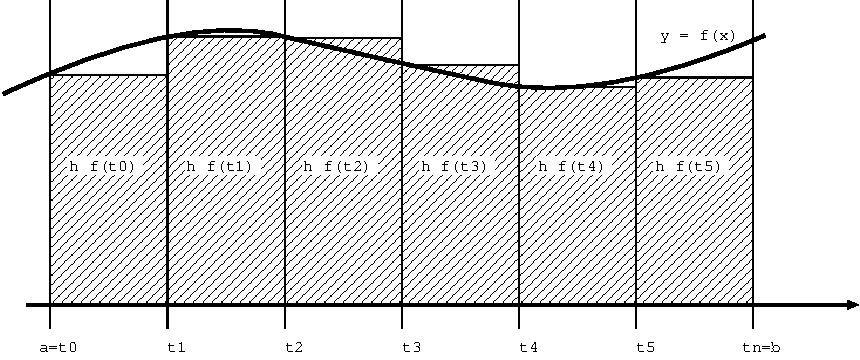
\includegraphics[width=.7\textwidth]{taylor-rectangulo.pdf}}

En otras palabras, calculamos la integral de la función que en cada intervalo $[t_{i-1},t_i)$ es constantemente igual a $f(t_{i-1})$.

Ya sabemos que $\Limn I_n^R = \int_a^b f(x)\, dx$ por lo visto en clase. Lo que nos preguntamos ahora es si podemos \emph{medir} o \emph{estimar} el error cometido al calcular $I_n^R$. La respuesta es positiva, y la da el siguiente 

\recuadro{
\begin{theorem}
 Sea $f:[a,b]\to \R$ una función con primera derivada continua en $[a,b]$. Si $\D M_1 = \max_{[a,b]}|f'|$, entonces
\[
 \Big| I_n^R  - \int_a^b f(x) \, dx \Big| \le \frac{M_1}{2} \frac{(b-a)^2}{n}.
\]
\end{theorem}
}

\begin{proof}
 Sea $n \in \N$ y sea $\pi_n$ la partición uniforme de $[a,b]$ en $n$ sub-intervalos de igual longitud $h := \Frac{b-a}{n}$, es decir, definimos $\pi_n = \big[a = t_0; t_1; t_2; \dots ; t_n = b\big]$ con $t_i = a + i\, h$. Observemos primero que
\begin{equation}\label{rect:uno}
\begin{aligned}
 \Big| I_n^R - \int_a^b f(x) \, dx \Big|
&=  \bigg| \sum_{i=1}^n \Big( h f(t_{i-1}) - \int_{t_{i-1}}^{t_i} f(x)\, dx \Big) \bigg] 
\\
&\le  \sum_{i=1}^n \Big| h f(t_{i-1}) - \int_{t_{i-1}}^{t_i} f(x)\, dx \Big|
\\
&=    \sum_{i=1}^n \Big| \int_{t_{i-1}}^{t_i} f(t_{i-1}) \, dx - \int_{t_{i-1}}^{t_i} f(x)\, dx \Big|
\\
&=    \sum_{i=1}^n \Big| \int_{t_{i-1}}^{t_i} \big( f(t_{i-1}) - f(x) \big) dx \Big|
\\
&\le    \sum_{i=1}^n   \int_{t_{i-1}}^{t_i} \big| f(x) - f(t_i) \big| dx .
\end{aligned}
\end{equation}
Intentemos ahora acotar cada uno de estos términos. Consideremos un intervalo $[t_{i-1}, t_i]$ de la partición, y observemos que si $x \in [t_{i-1}, t_i]$, entonces por el teorema fundamental del Cálculo se cumple que
\[
 f(x) - f(t_{i-1}) = \int_{t_{i-1}}^x f'(t)\, dt,
\]
y por lo tanto
\[
\big| f(x) - f(t_{i-1}) \big| = \Big| \int_{t_{i-1}}^x f'(t)\, dt, \Big|
\le \int_{t_{i-1}}^x |f'(t)| \, dt \le M_1 (x - t_{i-1}).
\]
Esto implica que
\begin{equation}\label{rect:dos}
  \int_{t_{i-1}}^{t_i} \big| f(x) - f(t_i) \big| dx  \le \int_{t_{i-1}}^{t_i} M_1 (x-t_{i-1}) \, dx
= M_1 \int_0^h u \, du = M_1 \frac{h^2}{2},
\end{equation}
donde hemos hecho la sustitución $u = x - t_{i-1}$, $du = dx$. Finalmente, de~\eqref{rect:uno} y de~\eqref{rect:dos} concluimos que
\begin{align*}
 \Big| I_n^R - \int_a^b f(x) \, dx \Big|
&\le   \sum_{i=1}^n   \int_{t_{i-1}}^{t_i} \big| f(x) - f(t_i) \big| dx 
\le \sum_{i=1}^n M_1 \frac{h^2}{2} 
\\
&= n M_1 \frac{h^2}{2} = n M_1 \frac{(b-a)^2}{2 \, n^2} = \frac{M_1}2 \frac{(b-a)^2}{n},
\end{align*}
que es lo que queríamos demostrar.
\end{proof}

\begin{obs}
 Si conocemos una cota para $M_1$, entonces podemos saber cuál es el valor de $n$ que debe tomarse para calcular la integral aproximada con un error dado.
\end{obs}

\begin{example}
 Supongamos que queremos calcular aproximadamente $\Int_0^2 e^{-x^2} \, dx$ con un error menor a $0.1$.

Si bien $f(x) = e^{-x^2}$ no parece una función muy complicada, no hay una fórmula conocida que dé su primitiva. Por eso recurrimos a un método numérico. Para saber qué valor de $n$ tenemos que tomar para lograr la precisión deseada, necesitamos conocer una cota superior para la primera derivada. Observemos entonces que $f'(x) = -2x e^{-x^2}$, y fácilmente deducimos que $|f'(x)| \le 4$ para $x \in [0,2]$. Entonces, para $n \in \N$, el teorema anterior nos dice que
\[
 \Big| I_n^R  - \int_0^2 e^{-x^2} \, dx \Big| \le \frac{4}{2} \frac{2^2}{n}
= \frac8n.
\]
Para asegurar un error menor o igual a $0.1$ debemos elegir $n$ tal que $\Frac{8}{n} \le 0.1$, o sea $n \ge 80$.
Para $n = 80$ la fórmula da $I_{80} = 0.89435$ (no se sugiere hacer a mano, sino usando una computadora, por ejemplo una planilla de cálculo o un programa como \MO). Por lo tanto
\[
 \Big| 0.89435  - \int_0^2 e^{-x^2} \, dx \Big| \le 0.1
\]
lo que a su vez implica que
\[
 0.89435 - 0.1 \le \int_0^2 e^{-x^2} \, dx \le 0.89435 + 0.1,
\]
es decir
\[
 0.79435 \le \int_0^2 e^{-x^2} \, dx \le 0.99435.
\]

Si quisiéramos cometer un error menor a $0.05$ (la mitad de la precisión anterior) ¿Cómo tendríamos que tomar $n$?

Sí, adivinaste, tendríamos que tomar $n=160$, ¡el doble!

Con un poco más de trabajo, podríamos haber demostrado que $|f'(x)| \le 1$ para $x \in [0,2]$, y en ese caso, habríamos estado seguros de que las precisiones indicadas se obtenían con 20 y 40 puntos respectivamente, un gran ahorro de trabajo, ¿no?
\end{example}



\subsection{Regla del trapecio}

La regla del trapecio es la siguiente: Para $n\in\N$, particionamos (de la misma manera que antes) el intervalo $[a,b]$ en $n$ sub-intervalos de igual longitud $h := \Frac{b-a}{n}$, es decir, definimos $\pi_n = \big[a = t_0; t_1; t_2; \dots ; t_n = b\big]$ con $t_i = a + i\, h$, y aproximamos $\Int_a^b f(x) \, dx = \sum_{i=1}^ n \int_{t_{i-1}}^{t_i} f(x)\,dx$ por la cantidad
\[
 I_n^T := \sum_{i=1}^n \frac{f(t_{i-1})+f(t_i)}2 (t_{i} - t_{i-1}) = \sum_{i=1}^n \frac{f(t_{i-1})+f(t_i)}2 h .
\]
Es decir, aproximamos cada integral en $[t_{i-1},t_i]$ por el área del \emph{trapecio} de altura $h$ y bases $f(t_{i-1})$ y $f(t_i)$.

\centerline{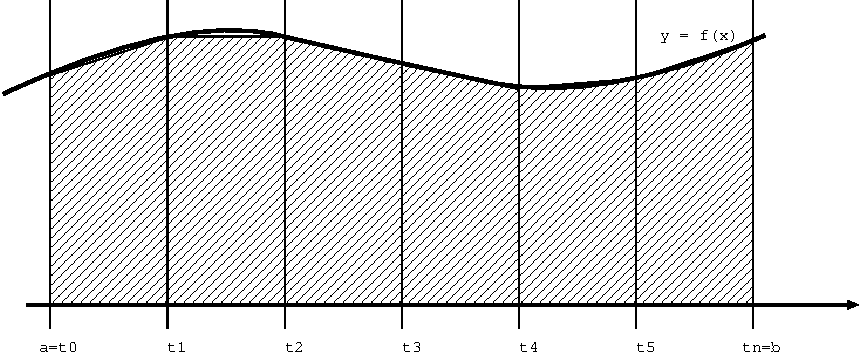
\includegraphics[width=.7\textwidth]{taylor-trapecio.pdf}}

En otras palabras, calculamos la integral de la función que en cada intervalo $[t_{i-1},t_i)$ es lineal y coincide con $f$ en $t_{i-1}$ y en $t_i$.

La gráfica nos invita a creer que el error cometido al calcular $I_n^T$ es menor que el que se comete al calcular $I_n^R$, y eso es \emph{en general} cierto, como lo confirma el siguiente 

\recuadro{
\begin{theorem}[Estimación del error de la regla del trapecio]
 Sea $f:[a,b]\to \R$ una función con segunda derivada continua en $[a,b]$. Si $\D M_2 = \max_{[a,b]}|f''|$, entonces
\[
 \Big| I_n^T  - \int_a^b f(x) \, dx \Big| \le M_2 \frac{(b-a)^3}{n^2}.
\]
\end{theorem}
}

\begin{proof}
 Sea $n \in \N$ y sea $\pi_n$ la partición uniforme de $[a,b]$ en $n$ sub-intervalos de igual longitud $h := \Frac{b-a}{n}$, es decir, definimos $\pi_n = \big[a = t_0; t_1; t_2; \dots ; t_n = b\big]$ con $t_i = a + i\, h$. Observemos primero que, si $\ell_i(x)$ es la función lineal cuya gráfica pasa por $(t_{i-1},f(t_{i-1}))$, y por $(t_i, f(t_i))$, entonces
\begin{equation}\label{trap:uno}
\begin{aligned} 
\Big| I_n^T - \int_a^b f(x) \, dx \Big|
&=  \bigg| \sum_{i=1}^n \Big( h \frac{f(t_{i-1})+f(t_i)}2 - \int_{t_{i-1}}^{t_i} f(x)\, dx \Big) \bigg] 
\\
&\le  \sum_{i=1}^n \Big| h \frac{f(t_{i-1})+f(t_i)}2 - \int_{t_{i-1}}^{t_i} f(x)\, dx \Big|
\\
&=    \sum_{i=1}^n \Big| \int_{t_{i-1}}^{t_i} \ell_i(x)\, dx - \int_{t_{i-1}}^{t_i} f(x)\, dx \Big|
\\
&=    \sum_{i=1}^n \Big| \int_{t_{i-1}}^{t_i} \big( \ell_i(x) - f(x) \big) dx \Big|
\le    \sum_{i=1}^n   \int_{t_{i-1}}^{t_i} \big| \ell_i(x) - f(x) \big| dx .
\end{aligned}
\end{equation}
Intentemos ahora acotar cada uno de estos términos. Para ello consideremos un intervalo $[t_{i-1}, t_i]$ de la partición, y definamos la función $g(x) = \ell_i(x)-f(x)$, que se anula en $x=t_{i-1}$ y en $x=t_i$, y por el teorema de Rolle existe $\xi_i \in (t_{i-1}, t_i)$ tal que $g'(\xi_i) = \ell_i'(\xi_i) - f'(\xi_i) = 0$. El teorema fundamental del cálculo nos dice que si $x \in (t_{i-1},t_i)$, entonces
\[
g'(x) = g(\xi_i) + \int_{\xi_i}^x g''(t) \, dt
  = \int_{\xi_i}^x g''(t)\, dt,
\]
como $\ell_i$ es lineal, $g''(t) = \ell_i''(t) - f''(t) = -f''(t)$ para $t \in (t_{i-1},t_i)$. Por lo tanto
\[
|g'(x)| = \Big|\int_{\xi_i}^x g''(t)\, dt \Big| = \Big|\int_{\xi_i}^x f''(t)\, dt \Big| \le |x-\xi_i| \, M_2 \le h \, M_2
\]
Esto implica que para $s \in (t_{i-1}, t_i)$
\begin{equation}\label{trap:dos}
 |g(s)| = |g(s) - g(t_{i-1})| = \Big| \int_{t_{i-1}}^s g'(x) \, dx \Big|
\le \int_{t_{i-1}}^s |g'(x)| \, dx \le M_2 h (s - t_{i-1}) \le M_2 h^2.
\end{equation}
Finalmente, de~\eqref{trap:dos} y de la definición de $g(x) = \ell_i(x) - f(x)$ se sigue que
\[
 \int_{t_{i-1}}^{t_i} \big| \ell_i(x) - f(x) \big| dx = \int_{t_{i-1}}^{t_i} \big| g(x) \big| dx
\le M_2 \, h^2 \, h = M_2 \, h^3,
\]
y por~\eqref{trap:uno} concluimos que
\[
 \Big| I_n^T - \int_a^b f(x) \, dx \Big| \le \sum_{i=1}^n \int_{t_{i-1}}^{t_i} \big| \ell_i(x) - f(x) \big| dx
\le M_2 \, h^3 \, n = M_2 \, \frac{(b-a)^3}{n^3} \, n = M_2 \, \frac{(b-a)^3}{n^2}.
\]
que es lo que queríamos demostrar.
\end{proof}

\begin{obs}
 En muchos libros, la fórmula de la regla del trapecio viene expresada como
\[
 I_n^R = = h \Big[ \frac{f(t_0)}{2} + f(t_1) + f(t_2) + \dots f(t_{n-1}) + \frac{f(t_n)}2 \Big].
\]
Fácilmente puede verse que es equivalente a la presentada al principio.
\end{obs}

\end{comment}


\subsection*{Ejercicios del capítulo~\getcurrentref{chapter}}


\begin{enumerate}
  \item Hallar el polinomio de Taylor $p_4$ de $f$, de orden $4$, alrededor de $x=0$ para las siguientes funciones:
\begin{multicols}{2}
  \begin{enumerate}
    \item $\D f(x)=x-\cos x$.
    \item $\D f(x)=\ln\big(\cos x\big)$.
  \end{enumerate}
\end{multicols}
\item Determinar $p_0(x)$, $p_1(x)$, $p_2(x)$, $p_3(x)$, (alrededor de $x=0$) para $f(x)=(x+1)^3$. 
\item Determinar el $n$-ésimo polinomio de Taylor $p_n$ de $f$, de orden $n$, alrededor de $x=0$ para las siguientes funciones:
\begin{multicols}{2}
  \begin{enumerate}
    \item $\D f(x)= e^{-x}$.
    \item $\D f(x)= \ln(1-x)$.
  \end{enumerate}
\end{multicols}

\item 
Calcular el polinomio de Taylor de grado 3 alrededor de $x=0$ de la función \[
  f(x)=\begin{cases}
      e^{1/x}, &\text{si } x<0,\\
      0, &\text{si }x\ge 0.
  \end{cases}
  \]
  \item Hallar la serie de Taylor de las siguientes funciones, alrededor del punto $a$ indicado:
\begin{multicols}{2}
  \begin{enumerate}
    \item $\D f(x) = e^{-x}$, $a = 0$.
    \item $\D f(x) = \frac1{1-x}$, $a = 0$.
    \item $\D f(x) = \ln (x+1)$, $a = 0$.
    \item $\D f(x) = \frac1x$, $a = 1$.
    \item $\D f(x) = \sqrt{x}$, $a = 1$.
  \end{enumerate}
  
\end{multicols}

\item Sea $f$ una función infinitamente diferenciable en $\R$, es decir, existe $f^{(n)}(x) = \frac{d^n}{dx^n}f(x)$, para todo $n\in 
\N$ y para todo $x\in \R$. 

Supongamos que además existe una constante $M>0$ tal que $|f^{(n)}(x)| \le M$, $\forall x\in [-a,a]$, para todo $n\in\N_0$, para algún $a>0$.

Demuestre que 
$\D f(x) = \sum_{k=0}^\infty \frac{f^{(k)}(0)}{k!}x^k$, para todo $x\in [a,a]$.

\item Consideremos la función $f(x)=\sen(x)$ en $\R$

\begin{enumerate}
\item Hallar el polinomio de Taylor de $f$ de grado $n$ para $n$ impar.

\item Hallar el polinomio de Taylor de $f$ de grado $n$ para $n$ par.

\item Demostrar que el resto $R_{n+1}(x)$ cumple $|R_{n+1}(x)| \le \frac{|x|^{n+1}}{(n+1)!}$.

\item  Demostrar que cualquiera sea $x \in \R$, se cumple que
\[ 
\sen(x) = \sum_{k=0}^\infty \frac{(-1)^k x^{2k+1} }{(2k+1)!}  
= x - \frac{x^3}{3!} + \frac{x^5}{5!} - \frac{x^7}{7!} + \frac{x^9}{9!} + \dots
\]
\end{enumerate}

\item Sea $f$ una función infinitamente diferenciable en $\R$, es decir, existe $f^{(n)}(x) = \frac{d^n}{dx^n}f(x)$, para todo $n\in 
\N$ y para todo $x\in \R$. 

Supongamos que además existe una constante $M>0$ tal que $|f^{(k)}(x)| \le M^k$, $\forall x\in \R$, $\forall k \in \N$.

Demostrar que 
$\D f(x) = \sum_{k=0}^\infty \frac{f^{(k)}(0)}{k!}x^k$, para todo $x\in \R$.
  
\item De una funci\'on $f$ con 4 derivadas continuas en $[-1,1]$ se sabe que
\[
f(0)=1,\quad f'(0)=-1,\quad f''(0)=2, \quad f'''(0)=0,
\]
y tambi\'en que $\D M_4=\max_{x\in[-1,1]}|f^{IV}(x)|\le 3$.

\begin{enumerate}
\item Utilizando el polinomio de Taylor de orden 3, calcular un valor aproximado de $\int_{-1}^1f(x)\,dx$
\item Estimar el error $|\int_{-1}^1 f(x)\, dx - \int_{-1}^1 p_3(x)\, dx|$.
\end{enumerate}

\item Se sabe que cierta funci\'on $f$ tiene cuatro derivadas continuas en
$[5,7]$ y que:
\[
f(6) = \frac12, \quad f'(6) = 0, \quad f''(6) = \frac14,
\quad f'''(6) = \frac18,\quad \max_{x\in[5,7]} |f^{(4)}(x)| \le 0.1.
\]
\begin{enumerate}
\item Utilizando el polinomio de Taylor de orden 3 alrededor de $x=6$
  calcular de manera aproximada $\int_5^7 f(x) \, dx$.
\item  Dar una estimaci\'on del error cometido al calcular la integral
    del \'\i tem anterior. Dar un intervalo donde seguramente se
    encuentre el resultado exacto.
\end{enumerate}

\item
Se sabe que cierta funci\'on $f$ tiene cuatro derivadas continuas en
$[-1,1]$ y que:
\[
f(0) = \frac12, \quad f'(0) = -\frac13, \quad f''(0) = -\frac14,
\quad f'''(0) = 0, \quad\text{y}\quad
\max_{x\in[-1,1]} |f^{(4)}(x)| \le 0.1
\]
\begin{enumerate}
\item Utilizando el polinomio de Taylor de $f$ alrededor de $0$, calcular de manera aproximada $\int_{-1}^1 f(x) \, dx$.

\item Estimar el error cometido al calcular dicha integral. Decir entre qu\'e dos valores se encuentra el valor verdadero de la integral.
\end{enumerate}

\end{enumerate}
  
